
%<><><><><><><><><><><><><><><><><><><><><><><><><><><><><><><><><><><><><><><><><><><><><>
 % Backgrounds
 %<><><><><><><><><><><><><><><><><><><><><><><><><><><><><><><><><><><><><><><><><><><><><>
\section{Backgrounds}

 \begin{figure}[tbh]
\begin{center}
%\includegraphics[height=5cm,viewport=250 180 0 360,clip=true]{CPP_production3}
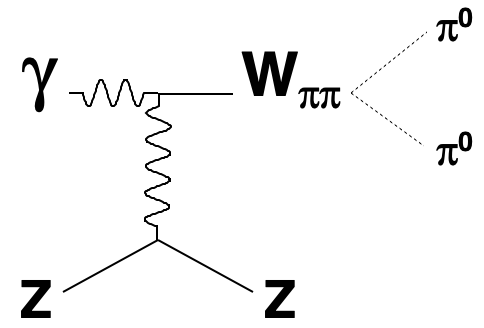
\includegraphics[height=5cm,clip=true]{figures/Diagram_Primakoff.png}
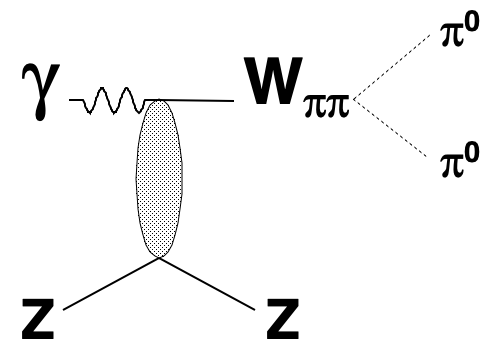
\includegraphics[height=5cm,clip=true]{figures/Diagram_hadronic.png}
\caption{Sketch of coherent two-pion production. Left) Signal: Primakoff mechanism, Right) Backgrounds: Other production mechanisms.
\label{fig:Diagram}}
\end{center}
\end{figure}

We first classify the various backgrounds and then describe them in more detail one at a time.
We note that two important backgrounds for the charged-pion polarizability experiment do not contribute in this experiment:
First, coherent $\rho^0$ photo-production is absent in this
experiment because the $\rho^0$ decay into the $\pi^0\pi^0$ channel is prohibited by I-spin conservation.  Second, $\mu^+\mu^-$ production is also not a factor for the neutral pion case.
We have the following categories of backgrounds:
\begin{itemize}
\item Coherent production: In this case, the target remains intact. Generically, one may classify the two-pion production
according to the sketches in Fig.\,\ref{fig:Diagram}. The left-hand diagram represents the exchange of a virtual photon with the nucleus, i.e. the Primakoff
mechanism. This mechanism is very long range and is affected minimally by the effects of shadowing or absorption.  This is the signal for the
experiment and our goal is to determine its cross section.
The right-hand diagram represents the exchange of a strongly interacting particle (or trajectory) and effectively results in the production of pions at the
surface of the nucleus. We note that for the neutral pion production, pion exchange is not allowed due to charge conjugation conservation, while 
for the charged pion case, single pion exchange is related to the axial anomaly ($\gamma \pi^0 \rightarrow \pi^+ \pi^-$).  When the interaction leaves the
nuclear target intact, the reaction is referred to as ``nuclear coherent'' and this is our most serious background. 
\item Incoherent production:  When the interaction produces two pions in the quasi-elastic scattering off a single
nucleon, the scattered target usually fragments into particles that range out in the target and are unobservable experimentally. This reaction occurs at larger $-t$ and is generally
kinematically distinct from the signal.
\item Any reaction that may be confused with the signal within the experimental resolution or limited acceptance:
 An example of this type of reaction is Primakoff production of $\eta$ mesons, where the $\eta\rightarrow \pi^0 \pi^0 \pi^0$  is
mis-reconstructed as a two-pion final state. 
\end{itemize}

\subsection{Coherent backgrounds}

 The largest coherent background is
from $f_0(500)$ and $f_0(980)$ photo-production.  The width of the
$f_0(980)$ is from 10 to 100~MeV, and can be eliminated from the data
by a cut on $\pi^0\pi^0$ invariant mass.  The $f_0(500)$ width is much
broader, from 400 to 700 MeV, with significant overlap in the
invariant mass region of interest.  Since the $f_0(500)$ is a scalar
particle with the same spin-parity as the $\gamma \gamma \rightarrow
\pi^0\pi^0$ final state near threshold, the azimuthal distribution of
the $\pi^0$ momentum or the $\pi^0\pi^0$ c.m. momentum relative to the
photon polarization plane does not differentiate between coherent
$f_0(500)$ production and the Primakoff reaction.  This is similar to
the Primex-$\pi^0$ experiment, where the dominant background was
nuclear coherent $\pi^0$ photo-production.  The approach used in the
Primex analysis was to measure the $\pi^0$ angular distribution,
effectively the $t$-distribution, then use theoretical calculations of
the angular distributions to separate out contributions from Primakoff
and nuclear coherent. The analysis of the $\pi^0\pi^0$ (NPP) reaction
will approximately parallel what was done for the Primex-$\pi^0$
analysis.

Primex data also showed that the nuclear coherent process is highly
suppressed for heavy nuclei.  The reason for the suppression is
$\pi^0$ absorption in the nuclear interior, making the coherent
production primarily a surface effect, i.e. proportional to $A$ and
not $A^2$.  For NPP it is expected that suppression of the nuclear
coherent will be stronger than that seen in Primex because two pions
are produced in NPP as compared to a single $\pi^0$ in Primex.  NPP
plans to run on a heavy nuclear target such as $^{208}$Pb.


\subsection{Incoherent backgrounds}


The inelastic and incoherent reactions that might contribute to the
data include
\begin{enumerate}[label=(\roman*)]
    \item nuclear coherent production of $\eta$ followed by $\eta\rightarrow \pi^0\pi^0\pi^0 \rightarrow \gamma\gamma\gamma\gamma(\gamma\gamma)$, where two of the six decay photons go unobserved
    \item $\gamma N \rightarrow N \pi^0\pi^0$
\end{enumerate}

The first reaction is an inelastic, coherent process, and as such
could produce a significant rate for a heavy nuclear target. Rejecting
events with extra gammas in the final state would suppress this
background.  The second reaction is an incoherent process, and is
small relative to coherent processes.  The Primex analysis showed that
incoherent reactions generally peak at large angles relative to the
Primakoff peak, and had a small effect on the extraction of the
Primakoff $\pi^0$ cross sections.